% !TEX root=/home/tavant/these/manuscript/src/manuscript.tex




\chapter{Parametric study of the dielectric characteristics}
\label{ch-2}
\headerchaptername{Dielectric parametric study}

\begin{Chabstract}
We use the PIC simulation code described in \cref{ch-1} to perform a parametric study over the two aspects of the dielectric walls\string: the secondary electron emission, and the modification of the electrostatic boundary condition.
We observe their impacts on the electron cross-field mobility, the electron mean temperature and the sheath characteristics.
The electrostatic boundary condition does not modify the results significantly.
On the other hand, the electron emission increases the near-wall mobility while decreasing the mean electron temperature, that reduces the importance of the \ac{ECDI} on the mobility.
A large discrepancy is observed between the sheath model of \cref{sec-sheath} and the PIC simulation results.
\end{Chabstract}



\minitoc


% 
% Structure \string:
% 
% {\bf II. Parametric study of the dielectric} 30 pages
% \begin{zzz}
%   This chapter takes the 1rst paper which uses Vivien's results.
% 
%   2.1 Fully metallic wall (no SEE, grounded).
% 
%   2.2 Impact of Dielectric layer without SEE
% 
%   2.3 Impact of SEE with grounded wall
% 
%   2.4 SEE and dielectric in the same time
% 
%   2.5 Discrepancy between $\mean{\Te}$, $\sigma_{PIC}$ and $\sigma_{theo} = \sigma_0 + (1 - \sigma_0) \frac{2 T_e}{\epsilon_0}$
% \end{zzz}


% !TEX root=/home/tavant/these/manuscript/src/manuscript.tex

\section{Simulation parameters}
  \label{sec-params}
  
  The simulation domain corresponds to the exit plane of the thruster.
  Hence, a neutral pressure $P_n$ of 0.1~mTorr and a plasma density $n_e$ of $\sn{1}{17}$ m$^{-3}$ are used.
  The fixed axial electric field and radial magnetic field are $E_z=\sn{2}{4}\,\volt\per\meter$ s and $B_r=200$ G, respectively.
  The rectangular \ac{2D} domain measures $L_r=2$~cm in the radial dimension and $L_{\theta}=0.5$~cm in the azimuthal direction.
  The axial length used for the convection is fixed at $L_z=1$~cm.
  It is important to note that the results shown in this chapter have been obtained at the beginning of my thesis, before the study of the convection presented in \cref{ch-1}.
  Hence, in this chapter we use the convection model of \citet{lafleur2016a}.
  However, we have validated at posteriori that the convection model used does not modify the results under the conditions studied.
  
  The numerical parameters are chosen to respect the stability criterion of \ac{PIC} simulation, and are presented in \Cref{parameters}
  
  \begin{table}[htbp] %PIC parameters
       \centering
       \ra{1.3}
       \caption{\label{parameters} Standard operating and numerical parameters used in the 2D PIC simulations of an HET.  The simulation results are given as representative values.}
       \begin{tabular}{@{}r c c c@{}} 
          \toprule
          {\bf Physical Parameter} & notation & Value & Unit \\
          \midrule
          Gas & & Xenon & - \\
          Domain dimensions & $L_{x} \times L_{y} \times L_{z}$ & $2.0 \times 0.5 \times 1.0$ & [cm$^3$] \\
          Radial magnetic field & $B_{0}$                    & $200$                 & [{G}] \\
          Axial electric field & $E_{0}$                    & $2 \times 10^{4}$     & [{Vm}$^{-1}$] \\
          Mean plasma density & $n_{0}$                    & $3 \times 10^{17}$    & [{m}$^{-3}$] \\
          Initial electron temperature & $\Te_{,0}  $               & $5.0$                 & [{V}] \\
          Initial ion temperature & $T_{i,0}   $               & $0.1$                 & [{V}] \\
          Secondary electron temperature & $T_{see}   $               & $1.0$                 & [{V}] \\
          Neutral gas pressure & $P_{n}     $               & $1.0$                 & [{mTorr}] \\
          Neutral gas temperature & $T_{n}     $               & $300$                 & [{K}] \\
          Neutral gas density & $n_{g}     $               & $3.22 \times 10^{19}$ & [{m}$^{-3}$]\\
          \midrule
          {\bf Simulation Parameter} &  &   &  \\
          
          Time step & $\Delta t  $                      & $4 \times 10^{-12}$ & [{s}] \\
          Cell size & $\Delta x = \Delta y = \Delta z $ & $2 \times 10^{-5}$  & [{m}] \\
          Number of particles per cell & $N/NG      $                      & $80$                & [{part/cell}] \\
          \midrule
          {\bf Typical quantities} &  &  &  \\ 
          Electron plasma frequency & $\omega_{pe}$               & $3.1 \times 10^{10} $  & [rad/s]\\
          Iopn plasma frequency & $\omega_{pi}$               & $36 \times 10^{6} $  & [rad/s]\\
          Electron cyclotron frequency & $\omega_{ce}$               &  $3.5\times 10^{9}$  & [rad/s] \\
          Electron Larmor radius & $r_{Le}$                    & 6$\times 10^{-4}$    & [m] \\
          \bottomrule
       \end{tabular}
    \end{table}
  
  
  The simulation is initialized with a uniform density of particles, following a Maxwellian distribution for temperature $\Te_{,0}$ and $\Ti_{,0}$ for the electrons and the ions respectively.
  
  
% !TEX root=/home/tavant/these/manuscript/src/manuscript.tex

\section{The base case}
  \label{sec-canonical}
  
  
  The {\it base} case corresponds to the case when the walls are grounded, and are fully absorbing. 
  It is the reference case that will be extensively described and commented.
  Then, it will be used as reference to analyze and quantify the effects of two characteristics of the dielectric walls on the studied discharges : the secondary electron emission, and the modification of the electrostatic boundary condition.
  
  \subsection{Initial phase of the simulation\string: \texorpdfstring{$t < 2\,\micro\second$}{ t < 2 microseconds} } \label{subsec-initlaphase}
  
  The initial phase of the simulation corresponds to the growth of the \ac{ECDI}, and the formation of the sheaths.
  Because of the growth of the instability, the electron transport increases as well, which increases the electron heating.
  The time scale of the sheath formation is governed by the ion inertia.
  It is roughly the same time scale as the saturation of the instability due to ion-trapping.
  
  \begin{figure}[hbt]
    \centering
    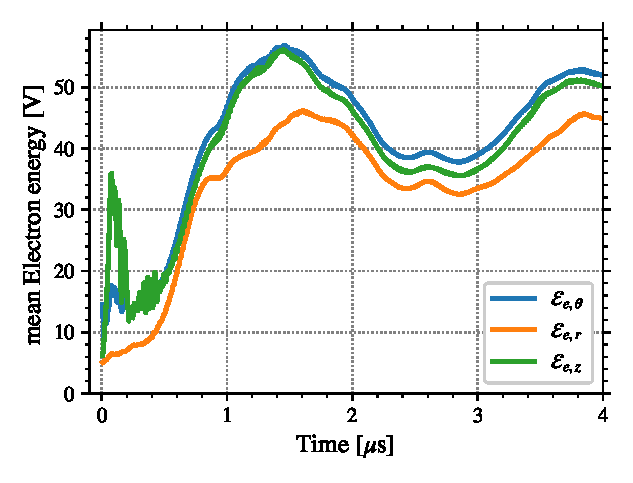
\includegraphics[width=\defaultwidth]{canonical_Te_start_directions}
    \caption{Temporal evolution of the electron mean kinetic energy decomposed over the three directions. Only the beginning of the simulation is shown.}
    \label{fig-canon_Te_strat}
  \end{figure}
  
  \Cref{fig-canon_Te_strat} shows the temporal evolution of the electron mean kinetic energy decomposed over the three directions, $\Ee_r, \Ee_{\theta}, \Ee_z$, such that
  \begin{equation} \label{eq-Ee_direction}
    \Ee_d = \frac{1}{n} \frac{1}{2} m_e \iiint_{\vect{v}}  v_{e,d}^2 f (\vect{v}) d^3v, \text{ with } d \in \{r, \theta, z  \}
  \end{equation}
  The mean kinetic energy is the sum of the thermal energy and the kinetic energy of the mean velocity.
  Because the electrons drift mainly in the azimuthal direction, we have
  \begin{equation} \label{eq-kinetic}
    \begin{cases}
      \Ee_r \simeq \frac{\Te_r}{2} \\
      \Ee_z \simeq \frac{\Te_z}{2} \\
      \Ee_{\theta} \simeq \frac{\Te_{\theta}}{2} + \frac{m_e}{2} \lp \frac{E_0}{B_0} \rp^2 \\
    \end{cases}
  \end{equation} 
  with $\frac{m_e}{2} \lp \frac{E_0}{B_0} \rp^2 \simeq  2.84\,\volt $.
  \nomenclature[Q]{\ensuremath{ \Ee}}{ Electron total kinetic energy, imposed of the thermal (or internal) energy and the kinetic energy of the mean velocity.  }
  We see that after some high frequency oscillations of $\Ee_{\theta}$ and $\Ee_z$ due to the cyclotron motion, the energies rise before stabilizing at $\Ee \simeq 45$V.
  The radial kinetic energy $\Ee_r$ is less than $\Ee_z$ and $\Ee_{\theta}$, but only by a small difference of $5\,\volt$, corresponding to roughly $10\%$.
  The small difference between the azimuthal and the axial kinetic energy is of the order of $2\,\volt$, as expected from the cyclotron motion of the electrons and \cref{eq-kinetic}.
  This means that the electrons are almost isotropic.
  
  
  \begin{figure}[hbt]
    \centering
    \begin{tabular}{@{} c c}
      \subfigure{time_r_mean_n}{a}{20, 20} &
          
      \subfigure{time_r_mean_phi}{b}{20, 20} 
    \end{tabular}
    \caption{Temporal evolution of the radial profile of the ({\bf a}) electron density and ({\bf b}) the plasma potential averaged azimuthally.}
    \label{fig-tx_n_phi}
  \end{figure}

  We can see in \Cref{fig-tx_n_phi} the evolution of the radial profile of the electron density on the plasma potential over the same period as \cref{fig-canon_Te_strat}.
  We observe on both quantities the formation of the sheath and the evolution toward a steady-state.
  
  \subsection{Saturated quasi steady-state\string: \texorpdfstring{$t \geq 2\,\micro\second$}{t > 2 microseconds}  }
  \label{subsec-stablephase}
  After the relatively fast rise of the plasma characteristics, the simulation reaches a quasi steady-state, as we can see in \Cref{fig-canon_Te_all}.
  We observe that after $t\simeq2\mus$ , the electron energy $\Ee$ starts to oscillate around a mean value.
  The oscillations are then damped and reach their minimum amplitude at  $t\simeq 7\mus$ and then remain with a small amplitude as shown on simulations carried out up to $25\,\micro\second$ in \cref{fig-canon_Te_all} (the origin of these oscillations has been discussed in \Cref{subsec-temp}).  
  
  
  \begin{figure}[hbt]
    \centering
    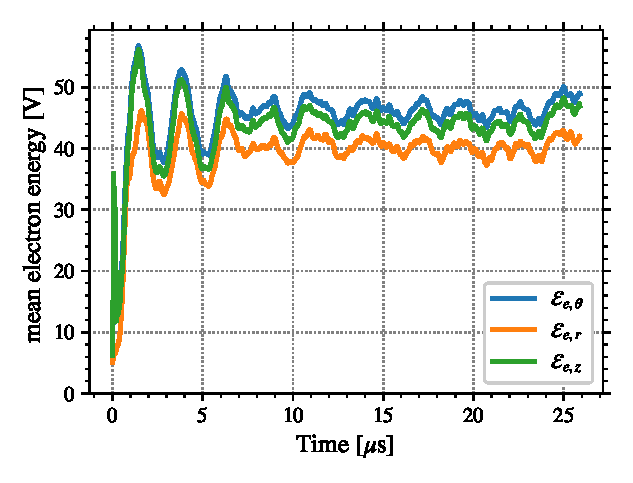
\includegraphics[width=\defaultwidth]{canonical_Te_all_directions_long}
    \caption{Temporal evolution of the electron mean kinetic energy decomposed over the three directions, similar to \cref{fig-canon_Te_strat} but for a longer period. We still see the difference between $\Ee_z$ and $\Ee_{\theta}$ due to the $E\times B$ drift, and the colder radial energy.}
    \label{fig-canon_Te_all}
  \end{figure}
  

  \Cref{fig-profiles} shows the azimuthally-averaged radial profiles of the electron and ion densities.
  The plasma is mostly quasineutral, except close to the walls, in the sheath, where the electron density falls more rapidly compared to that of ions.
  The sheath length can be roughly estimated to be $1\,\milli\meter$.
  The Debye length in our conditions is
  \begin{equation} \label{eq-debye}
    \lambda_D = \sqrt{\frac{\epsilon_0 k_b T_e}{n_e e^2}} \sim 0.4\,\milli\meter,
  \end{equation}
  which corresponds to the expected floating sheath length \citep{chabert2014} (a few $\lde$).
  
  \begin{figure}[hbt]
    \centering
    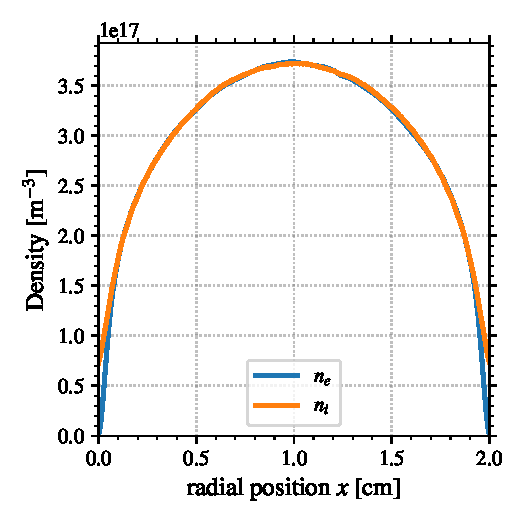
\includegraphics[width=\defaultwidth]{density_profile.pdf}
    \caption{Radial profile of the ion and electron densities at steady-state, averaged azimuthally and in time over the 5 last microseconds.}
    \label{fig-profiles}
  \end{figure}
  
  \subsection{Enhanced electron transport} \label{subsec-canonmue}
  As introduced in \cref{sec-transport}, the electron cross-field axial transport is characterized by the electron mobility
  \begin{equation} \label{eq-mobdef}
    \mob = \frac{u_{e, z}}{E_z}
  \end{equation}
  with $u_{e,z}$ and $E_z$ the electron mean axial velocity and the axial electric field, respectively.
  \nomenclature[Q]{\ensuremath{ \mob}}{ Electron mobility}
  \nomenclature[Q]{\ensuremath{ u}}{ Electron mean velocity}
  In \ac{PIC} simulations, $\mob$ is computed at each time step by
  \begin{equation} \label{eq-mobpic}
    \mobpic = \frac{1}{N E_z} \sum_N v_{e,z}
  \end{equation}

  \begin{figure}[hbt]
    \centering
    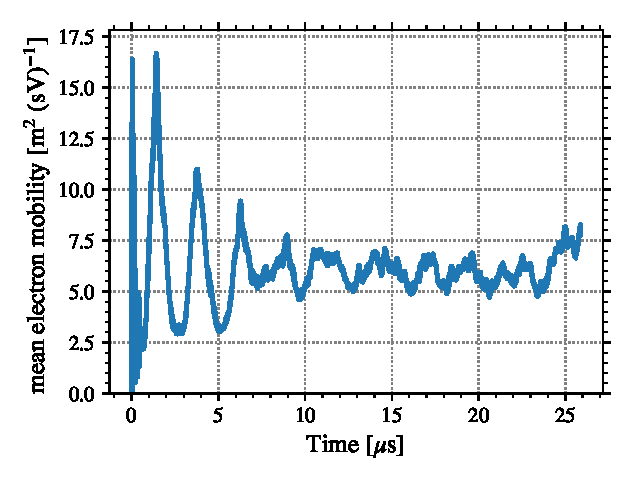
\includegraphics[width=\defaultwidth]{canonical_mu_all}
    \caption{Temporal evolution of the electron axial mobility computed in the \acs{PIC} simulation.}
    \label{fig-canon_mu}
  \end{figure}
  
  \Cref{fig-canon_mu} shows the temporal evolution of the electron mobility $\mobpic$ measured in the simulation with \cref{eq-mobpic}.
  We can see that it presents the same characteristics as the evolution of the electron energy $\Ee$ on \cref{fig-canon_Te_all}.
  We recall that the classical electron mobility from the collisional theory developed in \cref{eq-mobility} is \citep{lafleur2016a}
  \begin{equation} \label{eq-muclass}
    \mobcla = \frac{\nu_m \frac{e}{m_e}}{\oce^2 + \nu_m^2}
  \end{equation}
  with $\nu_m$ the electron-neutral  collision frequency and \oce{} is the electron cyclotron frequency.
  In the conditions of \cref{parameters}, $\mobcla \simeq 0.8$ \square\meter(sV)$^{-1}$.
  
  The measured electron mobility in the \ac{PIC} simulation is one order of magnitude larger than the classical mobility.
  In the present case, as no electron is emitted from the wall, the enhancement can only come from the instabilities present in the plasma.

  % K_ex = 2 10^-13
  % n_g = 1e19
  % wce = q B / m
  The oscillations can be seen in \cref{fig-2dschemat}, which shows the azimuthal electric field observed at $T=4\,\micro\second$.
  It clearly features the oscillation of wavelength of the order of 1~mm, as observed in \citet{heron2013}, and \citet{janhunen2018}.
  \Cref{fig-exampleECDI} shows the temporal evolution of the azimuthal electric field measured at the center of the channel.
  We can see that the instability rises and saturates quickly.
  Then, the oscillation remains quite stable.
  The Fourier Transform of the electric field presents a clear maximum at $14\,\mega\hertz$.
  The theoretical frequency of the \ac{ECDI} instability is \citep{lafleur2017}
  \begin{equation} \label{eq-maxfeq}
    f_{\rm max} = \frac{\omega_{pi}}{\sqrt{3}} \simeq 21 \,\mega\hertz,
  \end{equation}
  which gives a relatively good agreement with the oscillation observed.
  The \ac{ECDI} instability was the subject of \Cref{ch-5}, hence it will not be further discussed here.
  
  
  \begin{figure}[hbt]
    \centering
    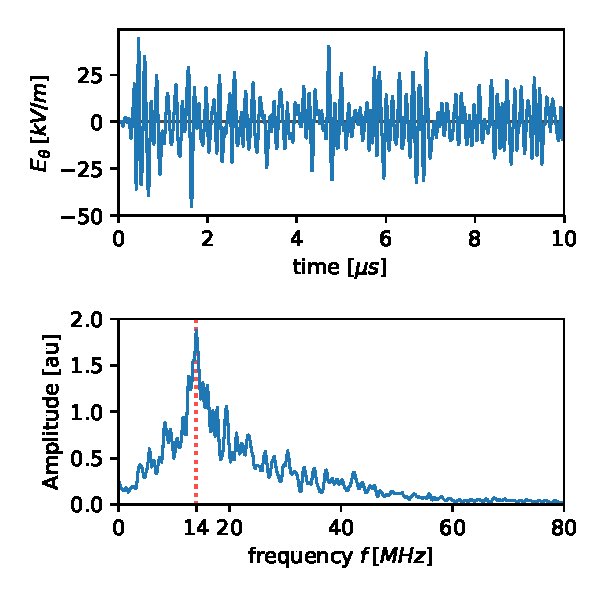
\includegraphics[width=\defaultwidth]{time_and_FFT}
    \caption{Azimuthal instability\string: temporal evolution of the azimuthal electric field at the center of the simulations, and its frequency spectrum computed by \acs{FFT}. The frequency for which the amplitude is maximum is highlighted.}
    \label{fig-exampleECDI}
  \end{figure}
  
  The effective mobility $\mobeff$ is determined by the correlation term $<\dEt \dne>$ and the parameters of the simulations.
  The effective mobility at saturation $\mobeffsat$, using the hypothesis of saturation by ion-wave trapping, only needs the electron temperature $\Te$.
  We can see that the three values $\mobpic, \mobeff$, and $\mobeffsat$ are close from each-others.
  
  \begin{table}[!hbt]
  \ra{1.3}
    \centering
    \caption{Characteristics  measured in the simulation at $t=27\,\micro\second$.}
    \label{tab-canonical_mobility}
    \begin{tabular}{@{} r l @{}} \toprule
    Quantity & Value \\ \midrule
    Correlation $<\dEt \dne>$ & $\sn{6}{20}$ V/m${^4}$ \\
    Effective mobility $\mobeff$ from \cref{eq-eq_mobeffsimple_two} & 4.4 m$^2$(sV)$^{-1}$ \\
    Mobility saturation $\mobeffsat$ from \cref{eq-mobeffsat} & 3.3 m$^2$(sV)$^{-1}$ \\
    Measured mobility $\mobpic$ from \cref{eq-mobpic} & 6 m$^2$(sV)$^{-1}$\\
    \bottomrule
    \end{tabular}
  \end{table}
  

  
  
% !TEX root=/home/tavant/these/manuscript/src/manuscript.tex

\section{Modeling the dielectric layer }
  \label{sec-diel_layer}
  
  The first effect of the wall material studied is adding a layer of dielectric material with its own permittivity, as introduced in \Cref{sec-diel}.
  The simulation parameters are the same as in the canonical case, presented in \cref{sec-canonical}, but the plasma is separated from the ground wall by a dielectric layer of 3~mm.
  Hence, the distance between the grounded electrodes is $2.6\,\centi\meter$.
  The relative permittivity of the dielectric is $\epsr=25$.
  %% SEE runs 250et 257 ?? Ly=1cm, Diel avec et sans SEE
  
  \Cref{fig-diel_radial_Er} shows the radial profile of the radial electric field $E_R$ at $t=10\,\micro\second$ averaged in the azimuthal direction.
  The plasma domain starts at $r=0$ and finishes at $r=2\,\centi\meter$.
  We note the jump in the value of the electric field at the plasma-wall transition.
  This jump is due to the surface charge.
  We can also notice that in the dielectric layer, in $r < 0$ and $r > 2\,\centi\meter$, the radial electric field is close to zero, compared to the value in the sheath.
  
  \begin{figure}[hbt]
    \centering
    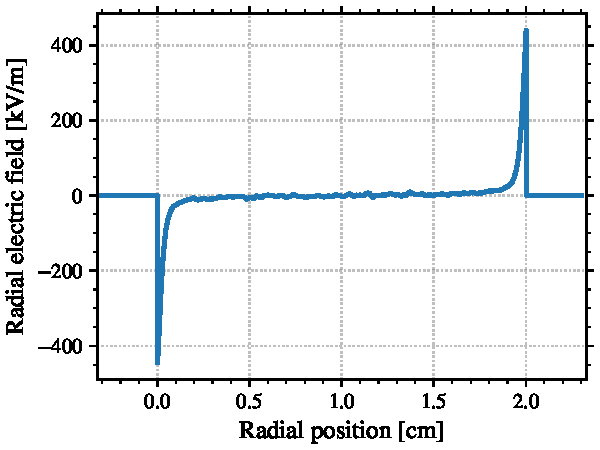
\includegraphics[width=\defaultwidth]{diel_average_radial_electric_field}
    \caption{Radial profile of the radial electric field $E_R$ averaged in the azimuthal direction at $t=10\,\micro\second$. The plasma domain starts at $r=0$ and finishes at $r=2\,\centi\meter$. The dielectric length is $L_{\\rm Diel} = 3\,\milli\meter$.  }
    \label{fig-diel_radial_Er}
  \end{figure}
  
  The next sections investigate the impact of the dielectric layer on the plasma characteristics, and highlight the plasma-wall interaction.
  
  \subsection{Effect of the dielectric layer} \label{subsec-effect_mob}
    
  
  The simulation results are qualitatively the same as in the case without the dielectric layer.
  As an example, \Cref{fig-mod_diel_comp} shows the temporal evolution of the axial electron mobility with and without the dielectric layer.
  We see that the results for the electron temperature and mobility are similar.
  The low amplitude oscillation of the case with the dielectric decreases slightly slower.
  
  \begin{figure}[hbt]
    \centering
    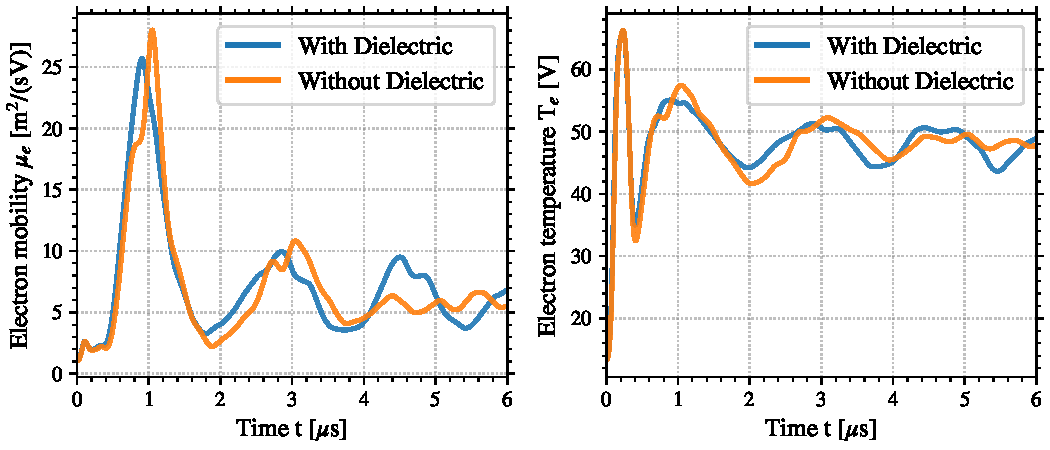
\includegraphics[width=\textwidth]{Dielectric_noSEE_temporal.pdf}
    \caption{Temporal evolution of the axial electron mobility (left), and the electron temperature (right) with and without the dielectric layer modeled.}
    \label{fig-mod_diel_comp}
  \end{figure}

  
  \subsection{Near-wall and in-wall parameters} \label{subsec-nearwall}
    In this section, we focus on the surface charge and the near-wall electric field.
    \Cref{fig-sigma_time} shows the temporal evolution of the surface charge at one point of the wall.
    The position has been chosen to be the center ($L_{\theta} = 0.25$~cm) of the lower wall, but the observations are similar at other positions.
     
    \begin{figure}[hbt]
      \centering
      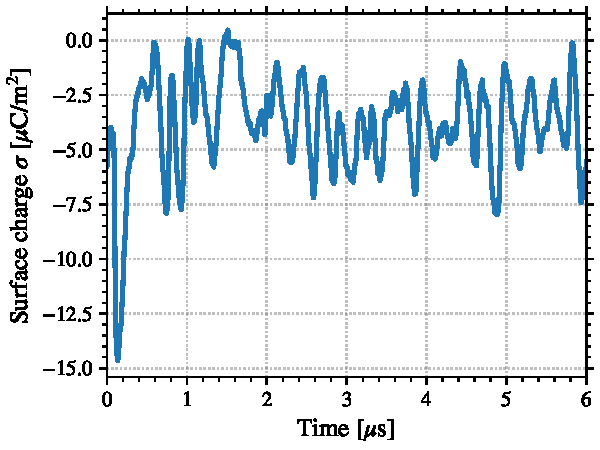
\includegraphics[width=\defaultwidth]{temporal_sigma}
      \caption{Temporal evolution of the surface charge $\sigma$ at one position of the lower dielectric wall}
      \label{fig-sigma_time}
    \end{figure}

    We can see on \cref{fig-sigma_time} that the value of the surface charge start by decreasing significantly (increasing in absolute value), due to the hot electrons that reach quickly the walls.
    Then, $\sigma$ growth and oscillates around a mean value close to $-3.5 \,\micro\coulomb/\square\meter$ and with an amplitude of approximately $1.2 \,\micro\coulomb/\square\meter$.
    
    \cref{fig-indiel} shows the azimuthal evolution of the radial electric field inside the dielectric layer.
    The electric field is given at three different positions ($r=-0.2, -0.9,$ and $-1.8\,\milli\meter$ away from the plasma-wall interface) to highlight its evolution.
    We can see that, even thought there is no charge in the dielectric, the amplitude of the electric field decreases when going further away from the plasma.
    This is due to the \ac{2D} Poisson equation, which smooth-out the inhomogeneity.
     
    \begin{figure}[hbt]
      \centering
      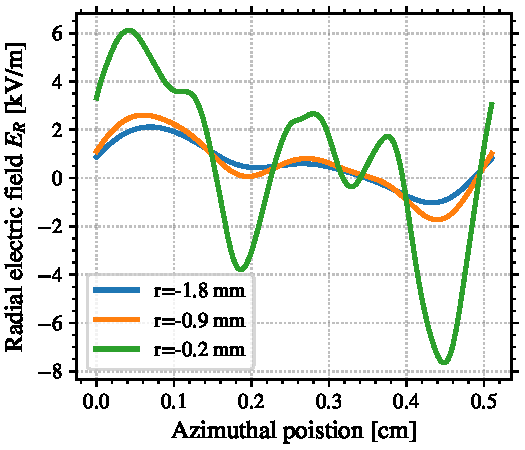
\includegraphics[width=\defaultwidth]{Radial_electric_feld_in_diel.pdf}
      \caption{Azimuthal evolution of the radial electric field inside of the dielectric layer at three different positions; the reference $r=0$ is the plasma-wall interface, the grounded electrode is located at $r=-3\,\milli\meter$.}
      \label{fig-indiel}
    \end{figure}

    
  \subsection{Dielectric model comparison} \label{subsec-modelcomp}
  
  \inlinenote{Anne: {\bf Beaucoup de remarques sur cette partie: pas assez claire, décrire plus les valeures observées, etc. Voir les notes sur le pdf (22 juillet)}}
  
  As introduced in \cref{sec-diel}, a simplified approach to model the effect of the surface charges on the plasma is to use a Neumann boundary condition \citep{taccogna2019}
  \begin{equation} \label{eq-neuman}
    E_r = \frac{\sigma}{\epsilon_0}.
  \end{equation}
  \Cref{eq-neuman} uses two approximations\string:
  \begin{itemize}
    \item one dimensional
    \item No electric field in the dielectric
  \end{itemize}
  We have already seen in \cref{fig-indiel} that the electric field in the dielectric is not zero, but instead it oscillates in respect to the azimuthal instability present in the plasma.  
  \Cref{fig-spacial_comparaison} shows the radial electric field at the wall and compares it to would be obtained by \cref{eq-neuman}.
  We can see that the two values are of the same order of magnitude, close to $-500$~kV/m.
  However, the two values are not equal, as they oscillates around their mean value.
  We can see that the surface charge oscillates more than the actual electric field obtained by solving the Poisson equation.

\begin{figure}[hbt]
  \centering
  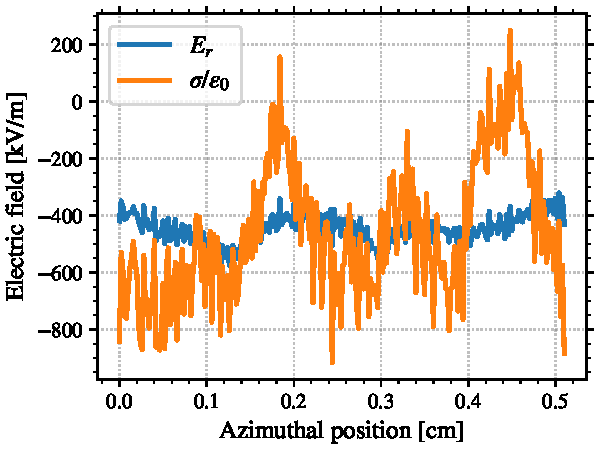
\includegraphics[width=\defaultwidth]{Radila_electric_field.pdf}
  \caption{Azimuthal evolution of the radial electric field at the plasma-wall interface and the electric field that would result from surface charge according to \cref{eq-neuman}.}
  \label{fig-spacial_comparaison}
\end{figure}
\renewcommand\subfigurewidth{0.45\textwidth}

  As a conclusion, we have observed that the dielectric layer does not change the simulation results much, but it can modify the surface processes.
  The model use here for the dielectric layer does not modify the performance of the simulation, while allowing to take into account the \ac{2D} effects.
  In this section, no secondary electron emission has been taken into account.
  In \cref{sec-fulldiel}, we will discuss the influence of using the simplified \cref{eq-neuman} in the case where secondary electron emission is important.

  
% !TEX root=/home/tavant/these/manuscript/src/manuscript.tex

\section{Impact of the radial boundary conditions on the oscillation}
  \label{subsec-BC}

  In \Cref{sec-DR-BC}, we discussed the choice of the radial wavenumber of the instability observed.
  Changing the radial electric boundary condition could affect the instability.
  Therefore, we discuss in this section  the impacts of the dielectric electrostatic boundary condition on the oscillation.
  We have seen in \Cref{sec-diel_layer} that the dielectric boundary did not affect the simulation results macroscopic.
  \Cref{fig-closswallosci} shows the radial evolution in the first few cells of the amplitude of the oscillation of the azimuthal electric field on the left, and the ion density on the right, with grounded (metallic) wall and dielectric wall.
  
  \begin{figure}[!hbt]
    \centering
    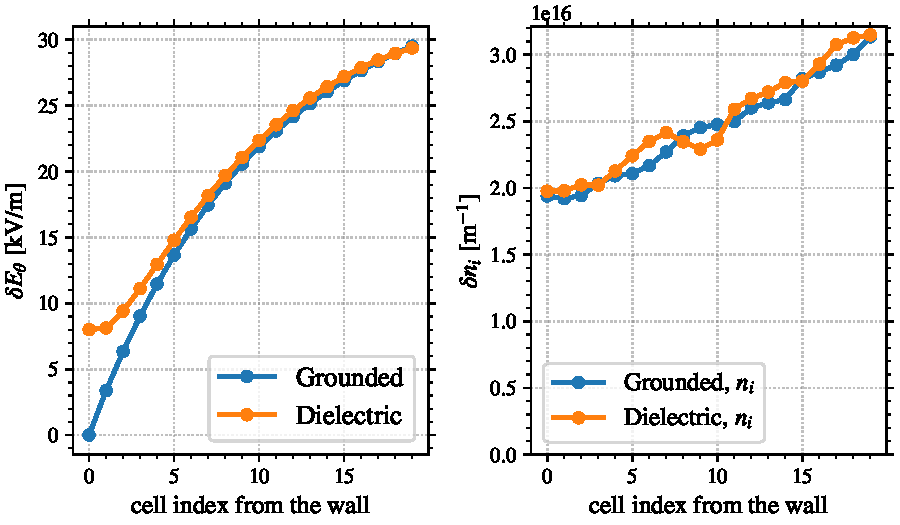
\includegraphics[width=\textwidth]{Ex_closewall.pdf}
    \caption{Radial evolution in the first cells of the amplitude of the oscillation of (left) the azimuthal electric field and (right) the ion density, with grounded (metallic) wall and dielectric wall.}
    \label{fig-closswallosci}
  \end{figure}
  
  We can see in \cref{fig-closswallosci} that the boundary condition does not affects the ion oscillations.
  This is consistent with the observation in \cref{subsec-kr} that the ion fluctuation was not affected by the wall.
  On the other hand, the azimuthal electric field has to go to zero when the wall is grounded.
  In contrast, using the dielectric boundary condition, the azimuthal electric field at the wall limit can be more than zero.
  Indeed, as seen in \cref{fig-indiel}, the amplitude of the azimuthal electric field decreases toward zero inside of the dielectric layer.
  
  Nevertheless, the difference in $E_{\theta}$ between the two boundary conditions quickly disappears inside the plasma domain.
  Indeed, after a dozen cells, corresponding to a few Debye lengths, the amplitudes of $\delta E_{\theta}$ are equal for both cases.
  Hence, the electrostatic boundary condition induces only minor differences in the instability and therefore the plasma discharge.
  
  
% !TEX root=/home/tavant/these/manuscript/src/manuscript.tex

\section{Effect of electron emission}
  \label{sec-see}
  
  In \Cref{sec-canonical}, the walls are not emissive.
  However, the dielectric ceramic used in \ac{HET} can emit electrons \citep{villemant2018,barral2003a}.
  The electron emission model used, introduced in \cref{sec-modelused}, has three parameters $\proba_0, \crover, \probamax$, such that the emission probability depends on the kinetic energy of the incident electron $\ek$ as
  \begin{equation} \label{eq-barral_second}
    \proba = \min \lp \proba_0 + (1 -  \proba_0) \frac{\ek}{\crover}, \probamax    \rp.
  \end{equation}
  
  The value of parameters are summarized in \cref{tab-tabe_parameters_see}.
  The crossover energy $\crover$ is varied from as low as 4~V, corresponding to a very emissive material, to as high as 200~V, a less emissive material.
  
  \begin{table}[hbtp]
  \ra{1.3}
    \centering
    \caption{Parameters of the electron emission probability model}
    \label{tab-tabe_parameters_see}
    \begin{tabular}{@{}ll@{}} \toprule
    Parameter & value  \\ \midrule
    $\proba_0$ & 0.5  \\
    $\probamax$ & 2.9 \\
    $\crover$   &  4  -- 200 V\\
    \bottomrule
    \end{tabular}
  \end{table}
  
  \begin{figure}[hbtp]
    \centering
    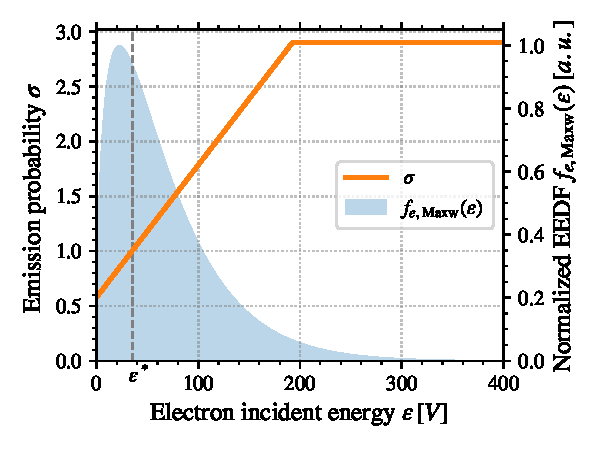
\includegraphics[width=\defaultwidth]{SEE_models}
    \caption{Illustration of the electron emission model of \cref{eq-barral_second} compared to a Maxwellian energy distribution function of temperature of 45~V, with $\crover=35.04$~V.}
    \label{fig-see_illustration}
  \end{figure}
  
  \Cref{fig-see_illustration} shows the electron emission probability for $\crover=35.04$~V compared to a Maxwellian \ac{EEDF} of temperature of 45~V.
  We can see that the saturation of $\proba$ at $\probamax$ happens only for the very high energy tail.
  In the simulation, we can only measure the average electron emission yield, also named emission rate, 
  \begin{equation} \label{eq-seeyield}
    \rate = \frac{\Gamma_{\rm emitted}}{\Gamma_{\rm incident}} = \frac{\iiint v_r \proba(\vect{v}) f(\vect{v}) d^3v}{\iiint v_r  f(\vect{v}) d^3v}.
  \end{equation}
  In general, \cref{eq-seeyield} cannot be calculated analytically.
  However, if we suppose that the \ac{EEDF} is Maxwellian and neglect the saturation at $\probamax$, \cref{eq-seeyield} yields
  \begin{equation} \label{eq-seemaxw}
    \ratemaxw(\Te) = \proba_0 + (1 - \proba_0) \frac{2 \Te}{\crover}.
  \end{equation}
  The saturation at $\probamax$ can be neglected as we have seen that it only affects a small part of the electron population, see \cref{fig-see_illustration}.
  \inlinenote{Add the exact calculation and the relative error ? \\Anne: oui. si trop long, a mettre en annexe.}
  
  \subsection{Impact of the electron emission of the mobility} \label{subsec-param-mob}
    
  The effects of the electron emission at the wall on the electron axial mobility are presented in \Cref{fig-mob-epsstar}.
  The measured mobility $\mobpic$ are shown, as well as the effective mobility $\mobeff$, the saturation estimate $\mobeffsat$ and the classical mobility $\mobcla$, defined in \cref{sec-transport} respectively by \cref{eq-mudef}, \cref{eq-defmobeff}, \cref{eq-mobeffsat} and \cref{eq-mobclas}.
  The values are averaged in time between $t=5 \mus$ and $t=10\mus$, and in space over the azimuthal and radial directions.
  \inlinenote{Anne: For epsilon=0, we have the values presented in section 2.2 without dielectrics.}
  \begin{figure}[hbtp]
    \centering
    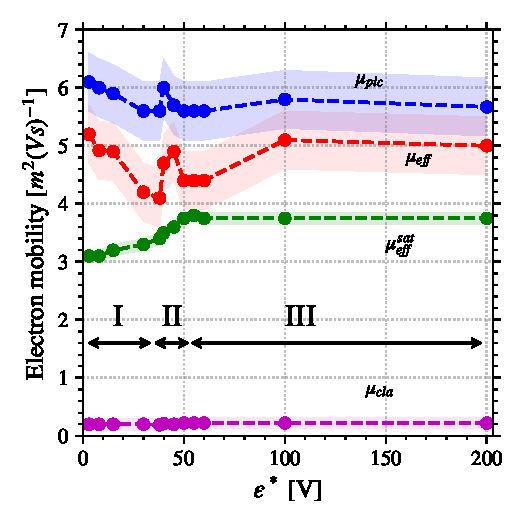
\includegraphics[width=\defaultwidth]{parametric_mobs_eps_complete}
    \caption{Evolution of the electron mobility as a function of the crossover energy $\crover$. In blue $\mobpic$ is the mobility measured in the simulations, while $\mobcla, \mobeff$ and $\mobeffsat$ in purple, red and green respectively are calculated with \cref{eq-mudef,eq-mobclas,eq-defmobeff,eq-mobeffsat}. The three regimes {\bf I, II} and {\bf III}, described in \cref{subsec-regimes} are identified.}
    \label{fig-mob-epsstar}
  \end{figure}
  \inlinenote{Units, in italic !}
  
  As expected, the classical mobility in  \cref{fig-mob-epsstar} is underestimated by more than one order of magnitude compared to $\mobpic$.
  The effective mobility $\mobeff$ and the effective mobility at saturation $\mobeffsat$  are much closer to $\mobpic$, with an underestimation of roughly 10\% and 30\% respectively.
  The mobility measured in the simulation does not evolve much with the electron emission, even for very high emission rate, i.e very low values of $\crover$.
  
  On the other hand, $\mobeffsat$ decreases slightly when $\crover$ decreases from around 40V to lower values.
  However, it still provides a reasonable approximation of the electron enhanced mobility, even with high electron emission rate. 
  
  \subsection{Near wall conductivity}
  
  The results presented in \cref{subsec-param-mob} are spatially averaged.
  However, the mobility coming from the  instability is expected to be higher where the instability is larger, hence at the center of the channel.
  On the other hand, the mobility due to wall emission is located close to the wall \citep{morozov1972}.
  
  \Cref{fig-radial-data} presents the radial profiles of the mobility measured in the \ac{PIC}  simulations without electron emission and for three values of $\crover$.
  On the left, the measured mobility $\mobpic$ is shown and on the right it is the effective mobility $\mobeff$ given by \cref{eq-defmobeff}.
  
  \begin{figure}[hbtp]
    \centering
    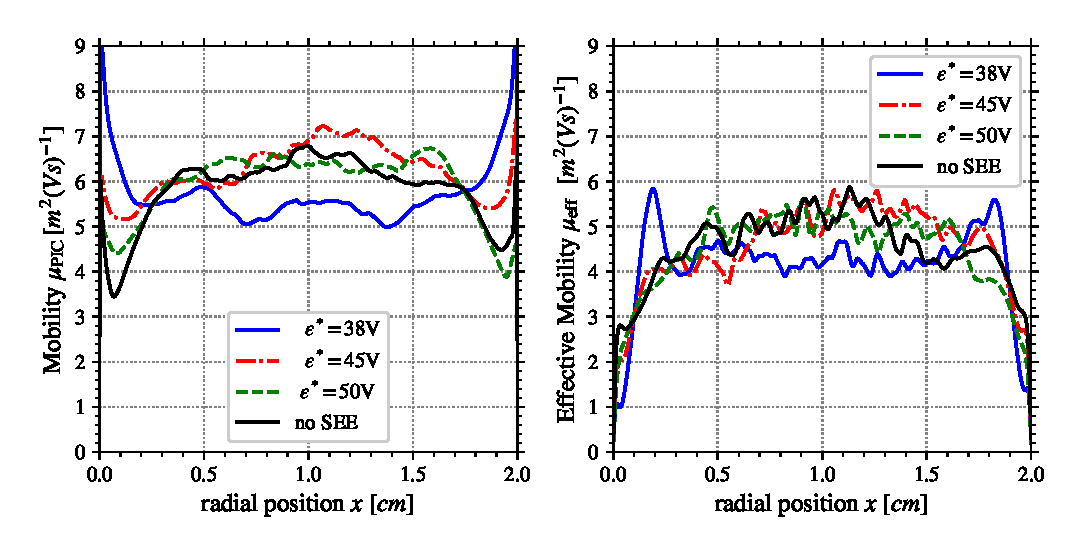
\includegraphics[width=\textwidth]{both_Mobility_SEE}
    \caption{Radial profile the electron mobility (left) measured in the \ac{PIC} simulations, and (right) given by \cref{eq-defmobeff}, for different wall emissivities. }
    \label{fig-radial-data}
  \end{figure}
  
  We can see in \cref{fig-radial-data} that the mobility measured $\mobpic$  in the center decreases by roughly 20\% as the emission rate increases.
  This observation is in agreement with $\mobeffsat$ observed in \cref{fig-radial-data,fig-mob-epsstar}.
  This is due the electron temperature $\Te$ which decreases from around $\Te=45$V at $\crover=200$V to $\Te=30$V at low $\crover$ (the evolution of $\Te$ can be seen in \cref{fig-Tevsproba}).
  
  On the other hand, the near wall mobility increases significantly on $\mobpic$ (almost by a factor of 2) with the increase of the electron emission.
  However, we do not see this evolution on $\mobeffsat$, meaning that it indeed comes from another physical mechanism than the \ac{ECDI}.
  
  
  \subsection{Three different regimes}
  \label{subsec-regimes}

  In \Cref{fig-mob-epsstar}, three regimes have been identified.
  Regime {\bf I} corresponds to low values of $\crover$ (lower than 35V), during which $\mobeffsat$ increases with $\crover$ but $\mobpic$ and $\mobeff$ decreases.
  Regime {\bf III} corresponds to high values of $\crover$ (higher than 50V), during which $\mobeffsat$, and  $\mobpic$ are roughlty constants, but $\mobeff$ increases slightly.
  Regime {\bf II} is a short transition regime, for $35 < \crover < 50$V.
  
  The different regimes are actually obvious when looking at the temporal evolution of the different variables.
  \Cref{fig-threeregimes}  presents the temporal evolution of the space average $\ratepic$ for three different
  values of $\crover$ , corresponding to three different regimes we have identified.
  In regimes {\bf I} and {\bf III}, $\ratepic$ reaches a steady state after a few microseconds.

  \begin{figure}[hbtp]
    \centering
    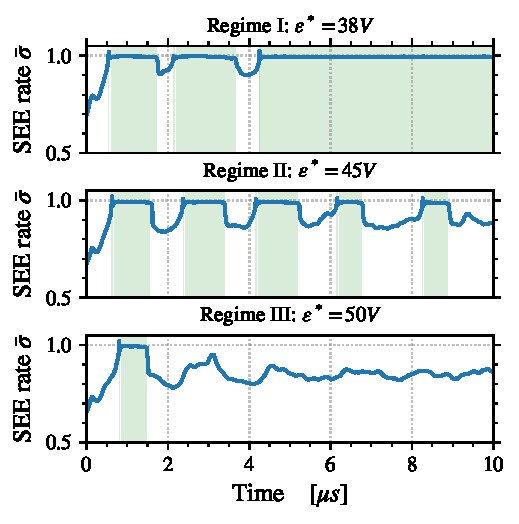
\includegraphics[width=\defaultwidth]{comparaison_3_regimes}
    \caption{Evolution as a function of time of the averaged electron emission rate $\ratepic$ in the three regimes observed (two stables, one with oscillations). The light green zones correspond to the periods when $\ratepic > \ratecr$}
    \label{fig-threeregimes}
  \end{figure}
  

  Regime {\bf I}, with low $\crover$, is characterized by a saturation of $\ratepic$ at a value between $\ratecr$ and 1, which leads to a non-monotonic potential profile.
  Regime {\bf III}, for higher $\crover$, is characterized by a steady state with a SEE rate lower than $\ratecr$.

  The transition between these two stable regimes (monotonic and non-monotonic sheath) passes by regime {\bf II}, an oscillating mode between the two stable regimes.
 As shown in \cref{fig-mob-epsstar}, regime {\bf II} is observed only in a narrow range of $\crover$.
 The oscillations of regime {\bf II} are shown in \cref{fig-threeregimes} up to $10\mus$ but have been observed for more than $40\mus$.
 Note that regimes {\bf I} and {\bf III} in \cref{fig-threeregimes} are obtained for $\crover = 38$~V and $\crover = 50$~V respectively, i.e. near the boundary of the unstable window (see \cref{fig-mob-epsstar}).
 Consequently, we observe a few oscillations before the steady-state is reached, as these cases are close to the bifurcation.
   
   
   The physical origin of the bifurcation can bee seen with the help of \cref{fig-dphivsTe}, which shows the evolution of the potential drop to the wall as a function of the electron temperature.
   It is computed using \cref{eq-seemaxw} for $\rate$ and \cref{eq-sheathhobbs} for the potential drop, which is summarized as 
   \begin{equation} \label{eq-dphi_vs_Te_Maxw}
     \begin{cases}
       \rate = \proba_0 + (1- \proba_0) \frac{2 \Te}{\crover} \\
       \dphi = \Te \ln \lp [1 - \rate] \sqrt{ \frac{m_i}{2 \pi m_e}}  \rp
     \end{cases}
   \end{equation}

   \begin{figure}[hbtp]
     \centering
     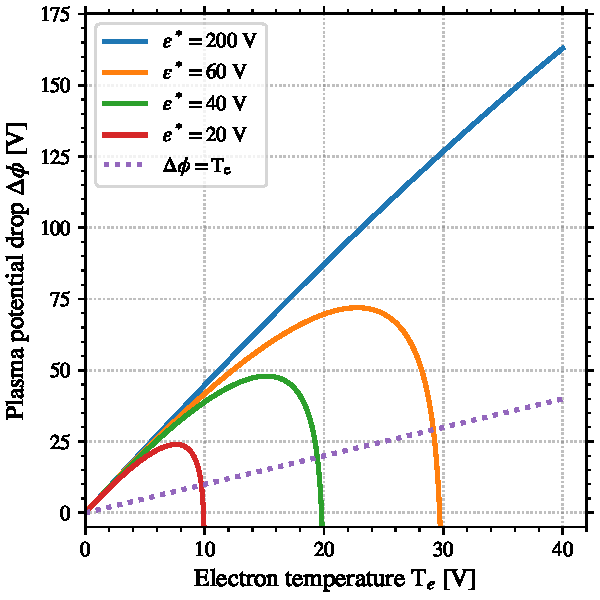
\includegraphics[width=\defaultwidth]{RSO_theo_sheath_bis}
     \caption{Plasma potential drop to the wall as a function of the electron temperature for different values of the cross-over energy $\crover$ using \cref{eq-dphi_vs_Te_Maxw}. The dashed line is $\dphi=\Te$. }
     \label{fig-dphivsTe}
   \end{figure}
   
   \Cref{fig-dphivsTe} shows the evolution of $\dphi$ as a function of $\Te$ obtained with \cref{eq-dphi_vs_Te_Maxw} using four different values of $\crover$. 
   We can see that, starting from low electron temperature, the potential drop increases with the electron temperature, resulting in a better screening of the electrons.
   This corresponds to regime {\bf III}.
   However, the $\dphi$ reaches a maximum, after which it drops sharply to zero and below.
   
   When the potential passes the maximum, the electrons are not screened by the sheath any more.
   Hence, the electrons reach the wall with a higher energy, resulting in a higher electron emission from the wall, hence a smaller potential drop.
   The sheath is unstable, and quickly attains a \ac{SCL} regime \citep{raitses2005}.
   
   In this regime, the sheath is not monotonic, and the model of \cref{eq-sheathhobbs} is no more valid, and the potential drop tends toward $\dphi \simeq \Te$ \citep{hobbs1967,goebel2008} \footnote{see \cref{sec-sheath} for more details}, shown in \cref{fig-dphivsTe}.
   This corresponds to regime {\bf I}.
   
   However, during regime {\bf I}, the electron power losses to the wall are very high, and they can exceed the gains.
   Hence, the electron temperature decreases.
   If $\Te$ decreases too much, the sheath can come back to the previous regime {\bf III}.
   The oscillations between regime {\bf I} and {\bf III} defines regimes {\bf II}.
      
   We have seen in \ref{fig-canon_Te_all} that without electron emission, $\Te$ is of the order of $45$~V.
   Using \cref{fig-dphivsTe}, we can expect to observe the transition between regime {\bf III} and {\bf II} for $\crover \gtrsim 60$~V, as for $\crover = 60$~V, the maximum of $\dphi$ is at $\Te\sim 25$~V, which is significantly lower than 45~V.
   The fact that regime {\bf II} appears at $\crover=50$~V can be explained because
   \begin{enumerate}
     \item a lower $\crover$ increases the electron losses, hence decreases the electron temperature at equilibrium,
     \item the electrons are not Maxwellian.
   \end{enumerate}
   
   The evolution of the temperature with $\crover$ is shown in \cref{fig-Tevsproba}.
   We can see that $\Te \simeq 45\,\volt$ for emission rate up to $\sigma = 0.8$, and decreases down to $\Te=30\,\volt$ for higher emission rates.
   Consequently, even if $\Te$ does indeed decreases when increasing $\crover$, it remains too large compared to the observations of \cref{fig-dphivsTe}.
   The impact of second point will be studied in \cref{ch-3}.
   
   
  
% !TEX root=/home/tavant/these/manuscript/src/manuscript.tex

\section{Validation of the sheath model }
  \label{sec-sheath_validation}
  
  The \ac{PIC} simulations used here do not need any sheath theory in order to model the plasma-wall interaction.
  Conversely, they rely on first principle models.
  Hence, they can be used in order to validate the sheath model introduced in \cref{sec-sheath} coming from the fluid theory.
  
  This sheath model links with \cref{eq-dphi_vs_Te_Maxw} the plasma potential drop $\dphi$ with the electron temperature $\Te$ and the electron emission rate $\rate$.
  \Cref{eq-seemaxw} can be used to estimate the electron emission rate given the mean electron temperature measured in the simulations, corresponding statistically to the plasma bulk temperature.   
  In the \ac{PIC} simulations, $\rate$ can be computed using \cref{eq-seeyield} by counting the number of electrons attaining the wall and emitted during a time-step.
  We note \ratepic this measurement.
  \vspace{1em}
   
  \begin{figure}[hbt]
    \centering
    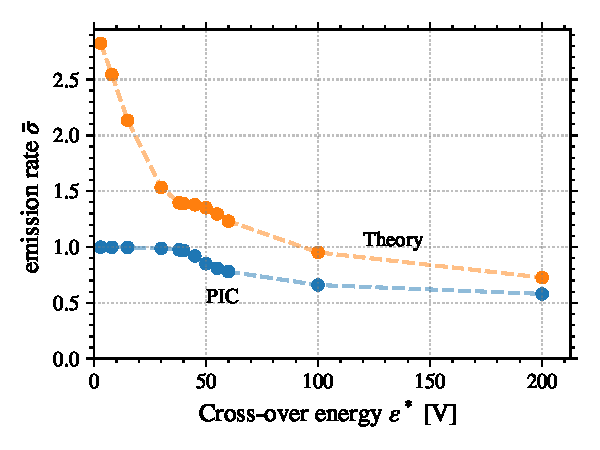
\includegraphics[width=\defaultwidth]{SEE_rates}
    \caption{Values of the electron emission rate $\ratepic$ (blue) measured in the \acs{PIC} simulations, and $ \ratemaxw$ obtained with \cref{eq-seemaxw} using the electron temperature shown in \cref{fig-Tevsproba}. }
    \label{fig-seeparamesMaxw}
  \end{figure}
  
  
  We can see in \Cref{fig-seeparamesMaxw} that the mean electron emission rate lies between 0.6 for large $\crover$ and 1 at low $\crover$.
  The saturation of $\ratepic$ at 1 for high emissivity ( $\crover < 50 \volt$) was not expected from \ratemaxw.
  Indeed, $\probamax$ is equal to 2.9, and the electron temperature in the bulk measured, when used in \cref{eq-seemaxw}, predicts a rate between 1.4 and 2.8.
  This discrepancy at low $\crover$ is due to the \ac{SCL} regime.
  \citet{hobbs1967} predicted that in this regime, a potential well forms such that a fraction of the emitted electrons return to the wall, in order to maintain the effective emission rate to $\ratecr\sim1$.
  However, for $\crover > 50 \volt$, the sheath regime described in \cref{sec-sheath} should be valid.
   
  \begin{figure}[hbt]
    \centering
    \begin{tabular}{@{} cc}
      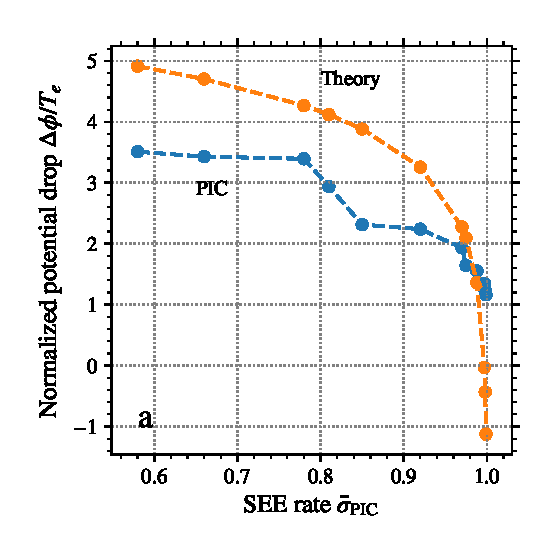
\includegraphics[width=0.45\textwidth]{phi_drop_6}
      &
      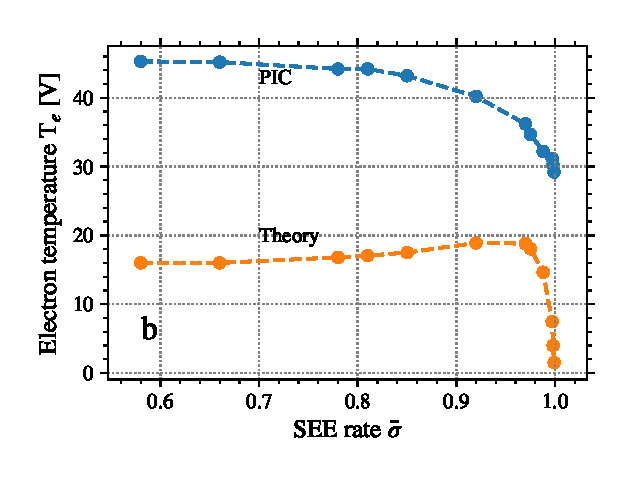
\includegraphics[width=0.45\textwidth]{Te_pic_2}
    \end{tabular}
    \caption{({\bf a}) Plasma potential drop to the wall normalized by the electron bulk temperature as a function of the electron rate, and ({\bf b}) the mean electron bulk temperature measured in the \acs{PIC} simulations as a function of the electron emission rate \rate, measured in the simulations, and the effective temperature expected from \cref{eq-Teeff}.  }
    \label{fig-Tevsproba}
  \end{figure}
  
  The electron temperature measured in the bulk of the simulation is presented in \cref{fig-Tevsproba}.{\bf b} for the same cases as in \cref{fig-seeparamesMaxw}.
  An \emph{effective} temperature that would correspond to the measured emission rate $\ratepic$ in \cref{eq-dphi_vs_Te_Maxw},
  \begin{equation} \label{eq-Teeff}
     \ratemaxw(\Te{}_{, eff}) = \ratepic \text{, hence } \Te{}_{, eff} = \frac{\ratepic - \sigo}{1 - \sigo} \frac{\crover}{2},
  \end{equation}
  is also given.
  We can see that when \rate increases, the electron temperature in the bulk $\Te$ monotonically decreases from 45V to around 30V.
  However, these values are not consistent with the measured emission rate \ratepic, even for $\crover > 50\volt$.
  The bulk electron temperature is much higher than the effective $\Te{}_{, eff}$ obtained to correctly predict the emission rate.

  \Cref{fig-Tevsproba}.{\bf a} shows the evolution of the potential drop to the wall measured in the \ac{PIC} simulation compared to the theory  \cref{eq-sheathhobbs} ).
  As expected by \cref{eq-dphi_scl}, $\dphi$ measured in the simulation saturates to $\Te$ for high emission rate ($\ratepic \sim 1$).
  However, we see that at low emission rate, the potential drop is significantly lower than expected.
  The sheath model of \cref{sec-sheath} used two hypotheses\string:
  \begin{itemize}
    \item Maxwellian distribution function to obtain $\ratemaxw$ from \cref{eq-seeyield},
    \item Isothermal electrons in the sheath.
  \end{itemize}
  These two hypotheses will be checked against the PIC simulations in the next chapter.

% !TEX root=/home/tavant/these/manuscript/src/manuscript.tex

\section{Full dielectric model }
  \label{sec-fulldiel}
  
  We have observed the effects of the electron emission and the electrostatic boundary condition separately in \cref{sec-diel_layer,sec-see}, respectively.  
  In \Cref{sec-see}, we observed three regimes depending on the emission rate.
  At high emissivity, the sheath is space-charge limited, resulting in an inverse sheath.
  At low emissivity, we obtain the standard sheath model with electron emission.
  The transition between the regimes passes by a oscillating regime.
  
  In \Cref{sec-diel_layer} we observed that when there is no emission, the dielectric boundary condition for the potential does not change the simulation results.
  In this section, we investigate the interaction between the two characteristics of the dielectric walls, especially with a high emission rate.
  More precisely, regime {\bf II} is the most interesting, as it features a complex behavior.
  Hence, we use $\crover=45\,\volt$ to study the impact of the dielectric layer combined with the electron emission.
  
  The dielectric layer thickness is $L_{\rm Diel} = 3\,\milli\meter$, and the relative permittivity of the dielectric is $\epsilon_R=25$.
  The dimensions of the plasma domain is not modified between the case with and without the dielectric layer.
  Instead, it is the width between the grounded electrodes that is increased.
  
  \subsection{Impact of the dielectric boundary condition on the mobility with electron emission}
    
    \Cref{fig-temporal_mu} shows the temporal evolution of the electron mobility measured in the simulation $\mobpic$ for both cases, with and without the dielectric layer.
    We can see that the two variables are quite similar, with similar mean values and oscillation.
    Interestingly, the beginning of the simulations, up to $t=3\,\micro\second$, are almost identical.
    After this, the values are not in phase.
    
    \begin{figure}[hbt]
      \centering
      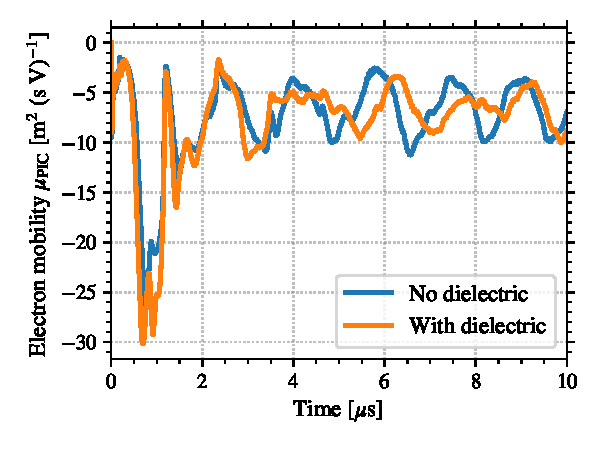
\includegraphics[width=\defaultwidth]{dielectron_yesSEE_mobility}
      \caption{Temporal evolution of the axial electron mobility measured in the \acs{PIC} simulation with and without the dielectric layer between the plasma and the grounded electrodes. The crossover energy is $\crover=45\,\volt$, the length of the dielectric layer is $L_{\rm Diel}=3\milli\meter$ and its relative permittivity is $\epsilon_R = 25$.  }
      \label{fig-temporal_mu} 
    \end{figure}
    
    
    \subsection{Plasma-wall interaction}

  
  \begin{figure}[hbt]
    \centering
    \begin{tabular}{@{} c c}
      \subfigure{see_diel_temporal}{a}{20,20} & 
      \subfigure{see_diel_space}{b}{20,20}
    \end{tabular}
    \caption{Comparison of the ({\bf a}) temporal and ({\bf b}) spatial evolution along the dielectric surface of the radial electric field at the wall calculated in PIC simulations compared to the electric field derived from the surface charge. }
    \label{fig-seediel_Er}
  \end{figure}
  \inlinenote{Anne: pas clair le choix des echelles de temps... Refaire ces figures avec les nouveaux resultats}
   
  \Cref{fig-seediel_Er} shows the ({\bf a}) temporal and ({\bf b}) spatial evolution along the dielectric surface of the radial electric field at the wall calculated in PIC simulations compared to the electric field derived from the surface charge, similarly  to \cref{fig-spacial_comparaison}.
  We can see that in contrast to the results of \cref{sec-diel_layer}, the two values are significantly different.
  The electric field measured in the \ac{PIC} simulation is rather uniform and constant, compared to the electric field at the surface calculated only based on the surface charge.
  Moreover, in \cref{fig-seediel_Er}.{\bf a}, we see that at around $t=2.1\,\second$, the electric field sign changes, meaning that the sheath passes from the \ac{SCL} regime {\bf I} to the normal regime {\bf III}, which is typical of regime {\bf II}.
  In contrast, the electric field derived from the surface charge does not shows this change of sheath regime.
  
  
  \begin{figure}[hbt]
    \centering
    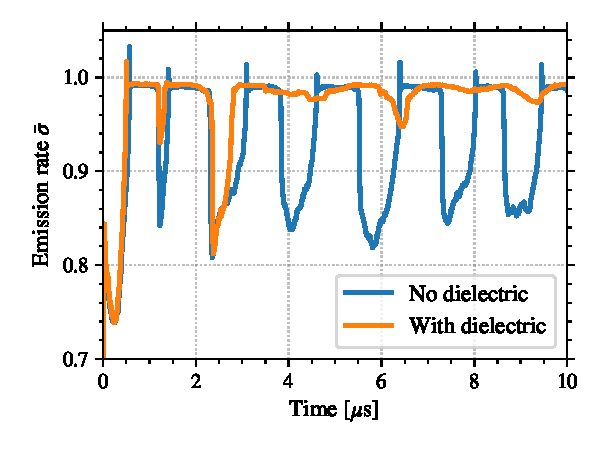
\includegraphics[width=\defaultwidth]{dielectron_yesSEE_SEErate}
    \caption{Temporal evolution of the mean electron emission rate $\ratepic$ for the same parameter $\crover=45\,\volt$, with and without the dielectric layer modeled.}
    \label{fig-rso_diel}
  \end{figure}
  
  \cref{fig-rso_diel} compares the temporal evolution of the mean electron emission rate $\ratepic$ for the same parameter $\crover=45\,\volt$, with and without the dielectric wall modeled.
  As previously, the dielectric width is $3\,\milli\meter$, and the electrodes are now $2.6\,\centi\meter$ apart (the geometry of the plasma domain is kept constant).
  We see that the oscillations occur for the two models.
  However, we can observe several differences.
  The first is the lower level of emission rate.
  When the walls are grounded, $\ratepic$ decreases at around $85\%$.
  Conversely, with the dielectric layer included, the emission rate does not decrease much below $95\%$.
  This results in a different overall mean emission rate, that can affect the particle and power balances, hence the mean electron temperature and the performance of the thruster.
  
  
  
  
  
% !TEX root=/home/tavant/these/manuscript/src/manuscript.tex

\section{Conclusion of the parametric study}
  \label{sec-conclusion_ch2}
  
  Using the \ac{PIC} simulation code introduced in \cref{ch-1}, we studied the effects of the dielectric walls on the discharge, and more precisely the effects on the electron axial mobility.
  To begin with, a \emph{base} case with metallic walls was defined and studied.
  The metallic walls correspond to grounded and non-emissive walls.
  For this reference case, we observed that the convection model used allows us to obtain a quasi steady-state.
  We observed an enhanced electron transport transverse to the magnetic field lines, because of the azimuthal instability.
  Both effects of the dielectric -- the electron induced electron emission and the electrostatic boundary condition -- were investigated.
  First, we  only modeled the dielectric boundary condition. Then, we studied only the electron emission. Afterwards, the two phenomena have been studied together.
  
  \subsubsection*{Electrostatic boundary condition}
  
  The electrostatic boundary condition is modeled by including in the domain of simulation the thickness of the wall ($L_{\rm Diel} = 3 \milli\meter$).
  Surface charges accumulate at the interface between the plasma and the wall.
  We observed that the modified boundary condition did not modify significantly the discharge and the axial cross-field electron mobility.
  Moreover, we saw that the boundary condition used results in a radial electric field $E_r$ of the same order of magnitude than the Neumann boundary condition of \cref{eq-neuman} but the spatio-temporal evolution is not identical.
  
  Indeed, when the secondary electron emission is modeled, the surface charges oscillates significantly compared to the radial electric field during the \ac{SCL} regime.
  As the dielectric model used here do not increase significantly the computational time, we recommend to use it instead of the Neumann boundary condition, that do not reproduce the same plasma-wall interaction.
  
  
  \subsubsection*{Electron induced electron emission}
  
  The electron  emission from the wall due to the impact of primary electron reaching the wall is modeled using the model described in \cref{sec-seemodel}.
  The value of the crossover energy $\crover$ is varied from a large value (low emissivity) to small values (high emissivity).
  We observed in the simulations that when the electron emission rate increases, the mean electron temperature decreases.
  This decreases the amplitude of the \ac{ECDI} at saturation, hence decreases the electron mobility in the plasma (see \cref{fig-radial-data}).
  However, electron emission induces \ac{NWC}, which almost doubles the electron mobility close to the wall when $\crover$ varies from $200\volt$ to $30\volt$.
  Consequently, the overall electron cross-field mobility is almost constant in our simulation.
  
  We observed in our \ac{PIC} simulations three different regimes depending on the values of $\crover$.
  For high values of $\crover$, the plasma stabilises with an emission rate $\ratepic < \ratecr$.
  When $\crover$ is small, we observe a stable configuration with $\ratepic \sim \ratecr$.
  Under these conditions, the sheath is space-charge limited.
  The transition between the two regimes is not stable, but instead passes by a bi-stable regime.
  In this third regime, the sheath jumps between the two stable regimes.
  

  \subsubsection*{Inconsistent sheath model }
  
  The simulation results have been compared to the sheath model of \citet{hobbs1967}.
  We observed a significant discrepancy between the \ac{PIC} simulations and the sheath model that comes from a fluid approach.
  In particular, the potential drop and the electron emission rate are both overestimated.
  These overestimations can lead to erroneous conclusion and prediction when using fluid models.
  Hence, a better understanding of the plasma-wall transition via the sheath is needed.
  
  The sheath model currently used is based mainly on two hypothesis
  \begin{itemize}
    \item Maxwellian electron distribution function
    \item Isothermal electrons in the sheath
  \end{itemize}
  
  Both hypotheses will be questioned in the next chapter.
  

